\documentclass{exam}
\usepackage[body={18cm, 25cm}]{geometry}
\usepackage[spanish]{babel}
\usepackage[utf8]{inputenc}					% include acents
%\usepackage[ansinew,latin1]{inputenc}
\usepackage[OT1]{fontenc}
\usepackage{amsmath,amssymb}
\usepackage{graphicx} % Para insertar y manejar imagenes
%\usepackage{subfig}
\usepackage{float}
\usepackage{caption}
\usepackage{subcaption}
\usepackage{enumerate}
\usepackage{enumitem} % Para usar [resume] en la enumeracion
\usepackage{cleveref}
\decimalpoint
%\usepackage{wrapfig}
%
%%% Nuevo Comando para cambio de pagina
\newcommand{\ask}{\textquestiondown}
\newcommand{\NuevaPagina}[1]{\newpage
\mbox{
\begin{minipage}{3cm}
	
\includegraphics[width=3cm]{images/logo.pdf} 
\end{minipage}
\begin{minipage}{14.7cm}
  \begin{flushright}
\hfill P\'agina #1 \hfill Parcial 03 \hfill Mayo 8 de 2015 \hfill C\'odigo: \rule{4cm}{0.3pt}
  \end{flushright}
\end{minipage}}\vspace{3pt}

\rule{18cm}{1.5pt}}

%%% COMIENZO DE DOCUMENTO %%%
\begin{document}
\pagestyle{empty}
%%% Encabezado
\mbox{
	\begin{minipage}{5cm}
		
\includegraphics[width=5cm]{images/logo.pdf} 
	\end{minipage}
	\begin{minipage}{13cm}
	\begin{center}
		\textsl{
		\textbf{\Large Escuela de Ingenier\'ias}\\
		\textbf{\large Mec\'anica del Medio Continuo Avanzada} \\
		\textbf{\large Tarea}
	}
	\end{center}
	\end{minipage}
}

\vspace{5mm}

\rule{\textwidth}{0.3pt} \\

%%% Fin del encabezado
%
En la figura \ref{fig:barra} se presenta una barra sobre la cual se aplica una fuerza $F_{x}$ en dirección $x$, que genera  un esfuerzo constante $\sigma_x$ sobre la cara donde está aplicada. La barra  está inicialmente separada de una lámina delgada de acero una distancia $d$, tal y como se muetra en \ref{sfig:barra2D}. El campo de desplazamientos para la barra mostrada es:\\\\
%
\begin{large}
	\hspace*{20mm} $u\left( x \right) = \dfrac{1}{E_1}  x \sigma_x$, \hspace*{10mm} $v=0$, \hspace*{10mm} $w\left( z \right) = - \dfrac{1}{E_2}  z (H^2 - y^2) \sigma_x$ \\\\
\end{large}

Donde $E_1 = 200000 kgf/cm^2$,   y $E_2 = 1000000$ $kgf$, $L = 1000 cm$, $H= 10 cm$.   $\sigma_x$ es el esfuerzo en dirección $x$ el cual tiene una variación en el tiempo deacuerdo a como lo muestra la  figura \ref{sfig:esfuerzo}.  \\\\

\begin{figure}[h]
	\centering
	\begin{subfigure}[l]{0.23\textwidth}
		\includegraphics[width=\textwidth]{images/barra.pdf} 
		\caption{Configuración inicial de la barra en 3D. Aplicación de la fuerza}
		\label{sfig:barra3D}
	\end{subfigure}	
	\hspace*{15mm}
	\begin{subfigure}[r]{0.23\textwidth}
		\includegraphics[width=\textwidth]{images/barrapared.pdf} 
		\caption{Vista en el plano $xz$. Separación inicial barra - lámina, d = 2.0 cm. $\phi = 45^\circ$}
		\label{sfig:barra2D}
	\end{subfigure}
	\hspace*{20mm}
	\label{sfig:barra}
		\begin{subfigure}[r]{0.30\textwidth}
		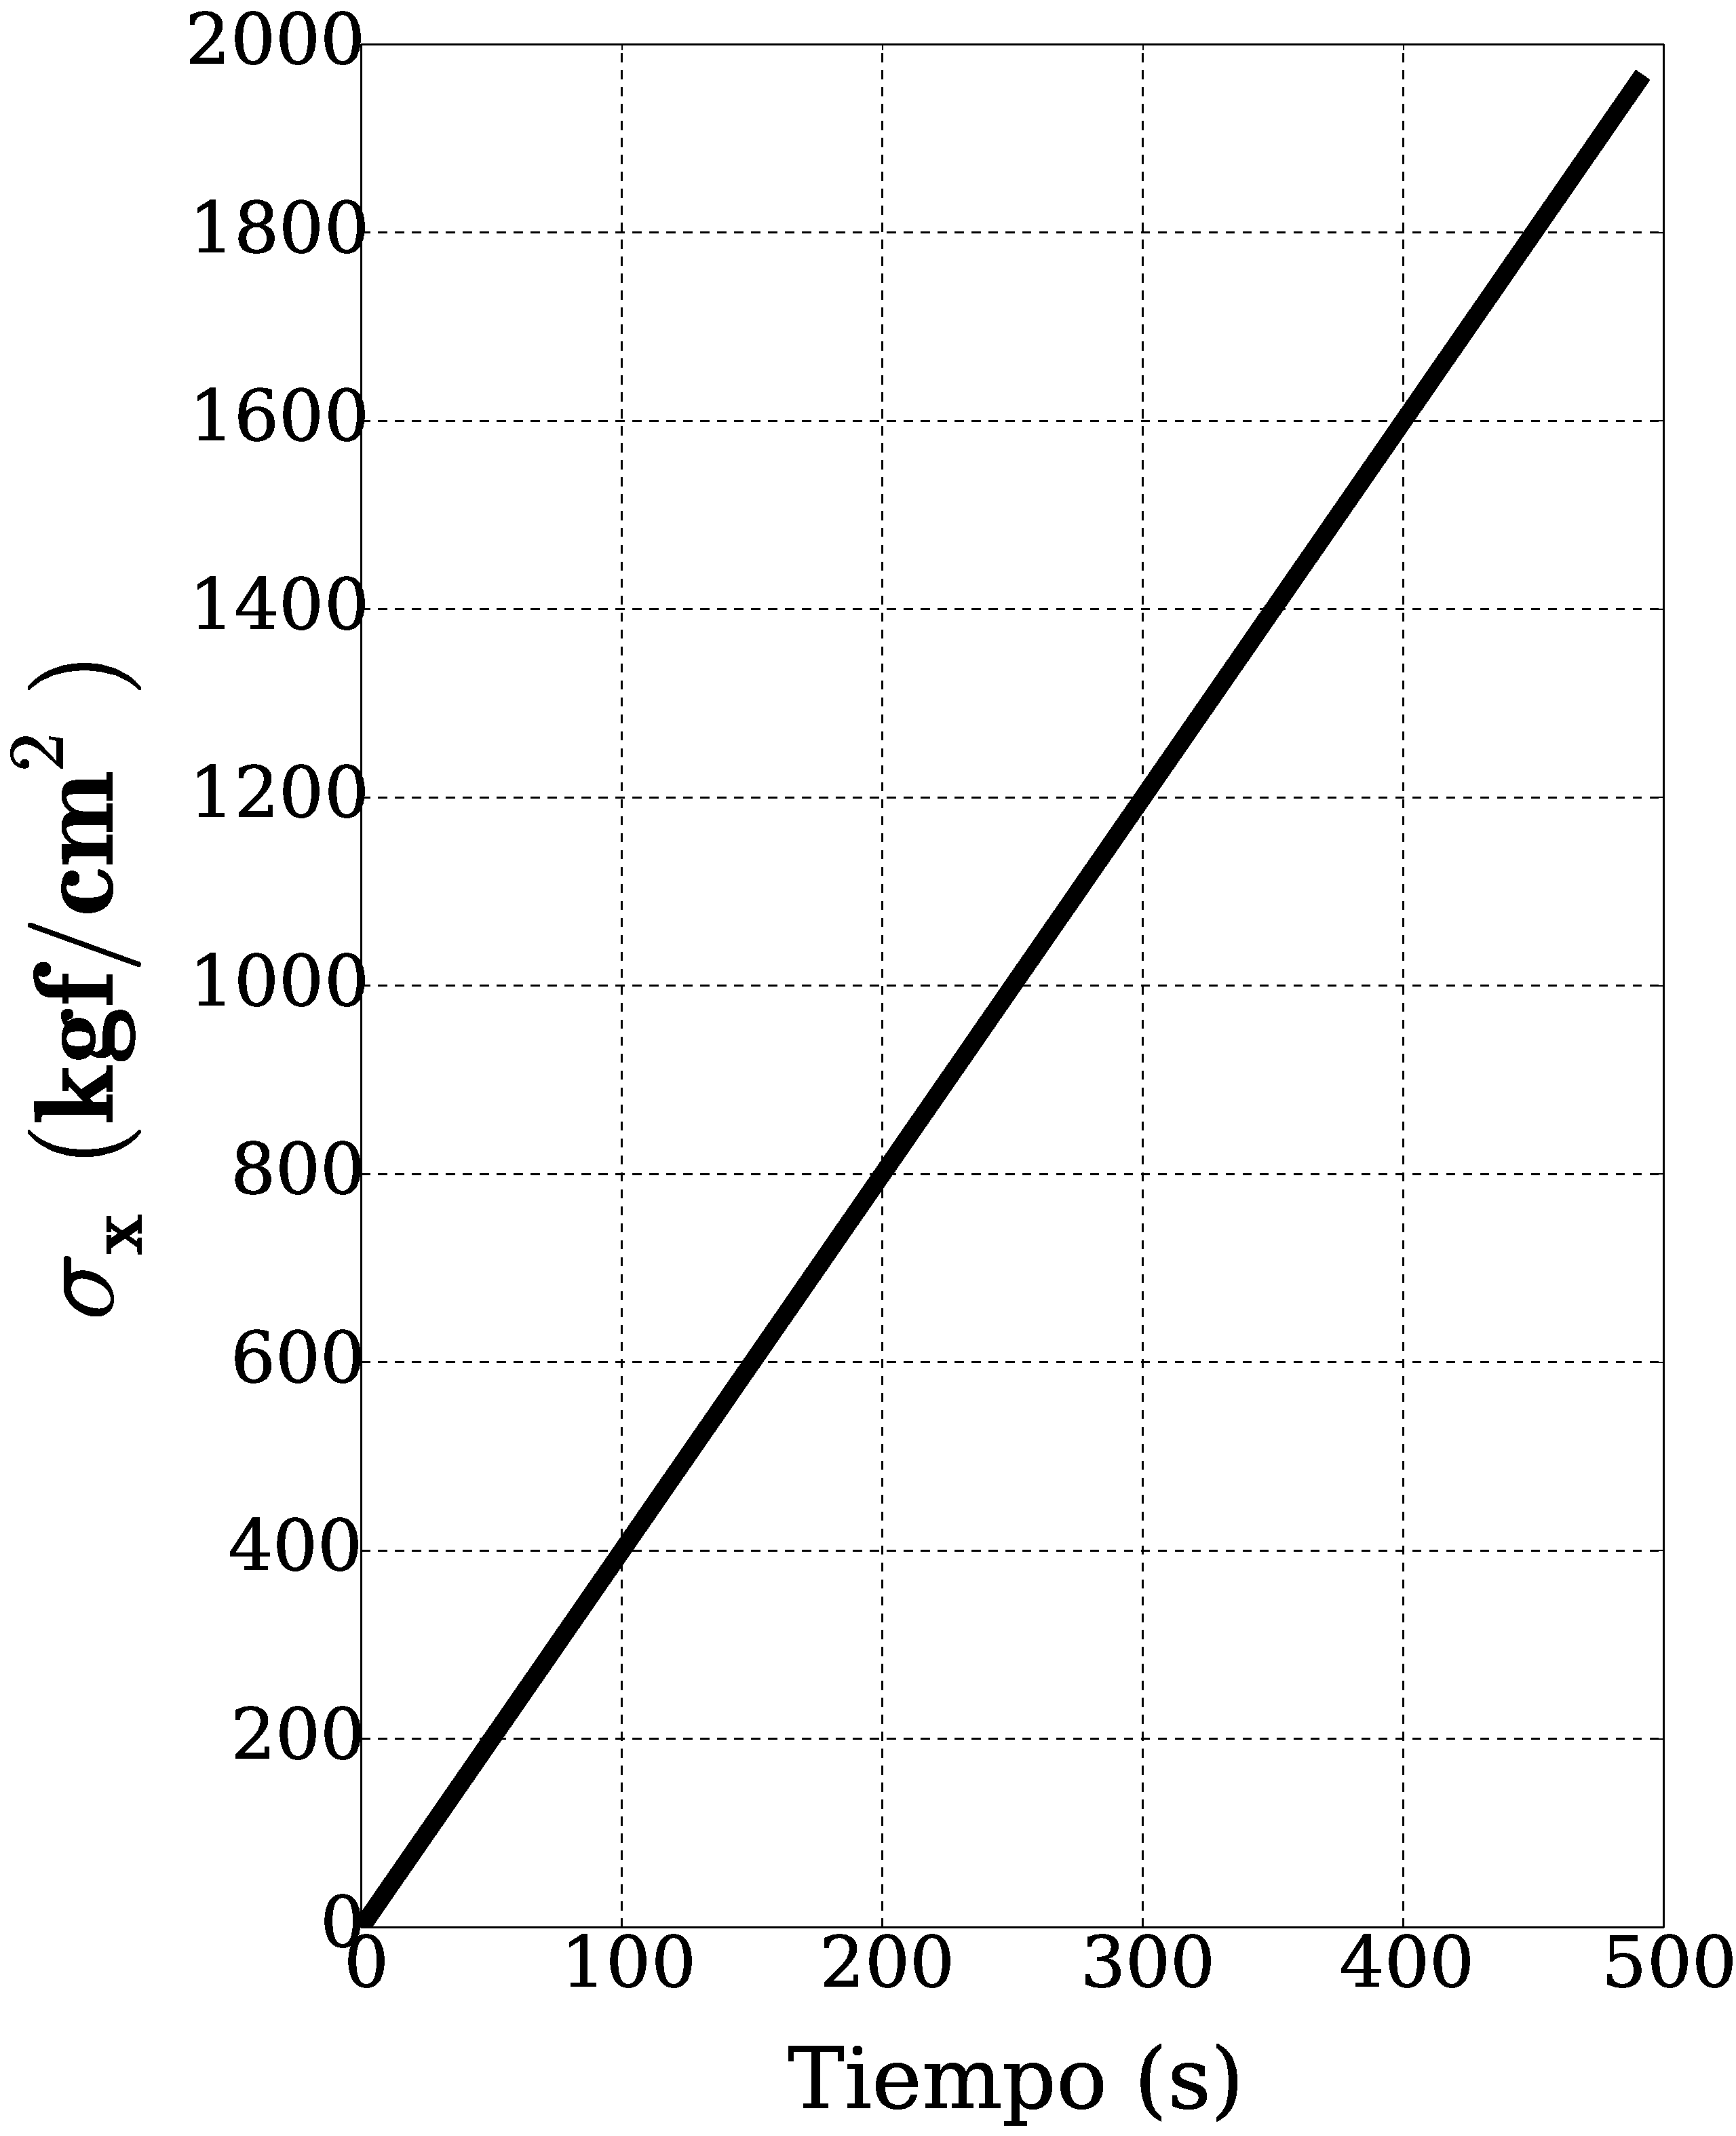
\includegraphics[width=\textwidth]{images/CurvaEsf.pdf} 
		\caption{Curva de esfuerzo.}
		\label{sfig:esfuerzo}
	\end{subfigure}
	\caption{Barra sometida a fuerza axial $F_{x}$}
	\label{fig:barra}
\end{figure}

\begin{enumerate}
	%
	\item $(10\%)$  Para el punto A de la barra con coordenadas  $(x,y,z) = (L, 0, H)$ grafique los desplazamientos $u$ y $w$ en función de tiempo. 
	\item $(50\%)$ Para los puntos de la cara $ z = 1.0 cm$ determinar el valor de la deformación angular máxima y en qué punto(s) se presenta. Hacer este cálculo cuando el valor del esfuerzo  $\sigma_x = 50  kgf/cm^2$  
	\item $(10\%)$  Dibuje la configuración deformada de la partícula para el punto de coordenadas $(x,y,z)=$ $(0,0,0)$ 

	\item $(30\%)$ Si el esfuerzo  $\sigma_x$ se incrementa  hasta que el punto  $A$ con coordenadas  $(x,y,z) = (L, 0, H)$ toque la lámina, determine el tiempo $t$  en el que la barra toca la lámina. ¿Cuáles serían las coordenas finales $x$, $z$ del punto A en ese instante? \\
	

\end{enumerate}
		
\textbf{Notas y parámetros de calificación:}
\begin{itemize}	
\item El documento PDF entregado debe ser autocontenido, es decir, que se lea y tenga sentido \textbf{por sí solo} sin tener que remitirse a otro documento que tenga los enunciados. Suponga que el documento va a ser leído por alguien que sabe mecánica, pero no tiene ningún contexto de la tarea. El no cumplmiento de esta condición causa una penalización del 30\% en la nota obtenida.

\item La tarea se debe entregar n formato profesional. Es decir, ecuaciones bien editadas y numeradas; figuras digitales con nombres de ejes, título, etc. Además de una redacción pertinente. El no cumplmiento de esta condición causa una penalización del 30\% en la nota obtenida.

\item La tarea se tiene que entregar antes del viernes 15 de marzo a las 2:00pm, hora de Colombia, en el buzón disponible en Interactiva Virtual. Las tareas que se entreguen por fuera del plazo no se tienen en cuenta.

\item Se debe realizar en grupos de máximo 3 personas.
\end{itemize}	
\end{document}